%%
%% This is a LaTeX template for writing Project Reports 
%% of the M Tech Programmes of APJAKTU. 
%% The template was developed by
%%     Dr V N Krishnachandran, 
%%     Vidya Academy of Science & Technology, 
%%     Thrissur - 680501.
%% Customized for ECE department, College of Engineering Trivandrum, by Christy James Jose, March 2024 
%% 
\documentclass[a4paper, 12pt, oneside]{book}
\usepackage{amsmath, amssymb}
\usepackage{graphicx, enumerate, multirow, fancyhdr}
\usepackage{mathptmx, anyfontsize, setspace}
\usepackage{indentfirst}
\usepackage{url}
\usepackage[total={5.5in, 9.5in},%
     top=1in, left=1.5in, includefoot]{geometry}%
\usepackage{hyperref}
\hypersetup{
    colorlinks=true,
    linkcolor=black,
    filecolor=blue,      
    urlcolor=blue,
    pdftitle={Overleaf Example},
    pdfpagemode=FullScreen,
    citecolor=blue
    }

\urlstyle{same}
%%
\setcounter{secnumdepth}{3}
%%
% Title of the project
\newcommand{\ttitle}[1]%
{\def\vtitle{#1}}%
% name of student
\newcommand{\nname}[1]%
{\def\vname{#1}}%
\newcommand{\rregisternumber}[1]%
{\def\vregisternumber{#1}}%

\newcommand{\nnamei}[1]%
{\def\vnamei{#1}}%
\newcommand{\rregisternumberi}[1]%
{\def\vregisternumberi{#1}}%

\newcommand{\nnameii}[1]%
{\def\vnameii{#1}}%
\newcommand{\rregisternumberii}[1]%
{\def\vregisternumberii{#1}}%

\newcommand{\nnameiii}[1]%
{\def\vnameiii{#1}}%
\newcommand{\rregisternumberiii}[1]%
{\def\vregisternumberiii{#1}}%
% Register Number of student
%\newcommand{\rregisternumber}[1]%
%{\def\vregisternumber{#1}}%
% Specialization
\newcommand{\sspecialization}[1]%
{\def\vspecialization{#1}}%
% File name of college emblem
\newcommand{\eemblem}[1]%
{\def\vemblem{#1}}%
% Department offering the BTech program
\newcommand{\ddept}[1]%
{\def\vdept{#1}}%

% name of the College
\newcommand{\ccollege}[1]%
{\def\vcollege{#1}}%
% First line of address of College
\newcommand{\aaddresslinei}[1]%
{\def\vaddresslinei{#1}}%
% second line of address of College
\newcommand{\aaddresslineii}[1]%
{\def\vaddresslineii{#1}}%
% Third line of address of College
\newcommand{\aaddresslineiii}[1]%
{\def\vaddresslineiii{#1}}%
% Name of Head of Department
\newcommand{\hhod}[1]%
{\def\vhod{#1}}%
% Name of Internal Supervisor
\newcommand{\gguide}[1]%
{\def\vguide{#1}}%
%project co -ordinator1
\newcommand{\pprojectco}[1]%
{\def\pprojectco{#1}}%

%project co -ordinator2
\newcommand{\pprojectcoii}[1]%
{\def\pprojectcoii{#1}}%


% Date
\newcommand{\ddate}[1]%
{\def\vdate{#1}}%
%%
%% Redefining chapter/section/sub-section commands
%%
\makeatletter
\def\@makechapterhead#1%
{%
   \vspace*{30\p@}%
   {%
      \parindent \z@ \centering \normalfont
      \ifnum \c@secnumdepth >\m@ne
         \if@mainmatter
            \fontsize{15.5}{20}\selectfont\bfseries% 
            \@chapapp\space \thechapter
            \par\nobreak
         \fi
      \fi
      \interlinepenalty\@M
      \fontsize{15.5}{20}\selectfont\bfseries% 
      \MakeUppercase{#1}\par\nobreak
      \vskip 20\p@
   }%
}%
%%
\def\@chapter[#1]#2%
{%
   \thispagestyle{empty} 
   \ifnum \c@secnumdepth >\m@ne
      \if@mainmatter
         \refstepcounter{chapter}%
         \typeout{\@chapapp\space \thechapter.}%
         \addcontentsline{toc}{chapter}%
         {\protect\numberline{Chapter \thechapter.\enspace  
             \MakeUppercase{#1}}}%
      \else
         \addcontentsline{toc}{chapter}{#1}%
      \fi
   \chaptermark{#1}%
   \addtocontents{lof}{\protect\addvspace{10\p@}}%
   \addtocontents{lot}{\protect\addvspace{10\p@}}%
   \if@twocolumn
      \@topnewpage[\@makechapterhead{#2}]%
   \else
      \@makechapterhead{#2}%
      \@afterheading
   \fi
}%
%%
\def\@makeschapterhead#1%
{%
   \vspace*{30\p@}%
   {%
      \parindent \z@ \centering
      \normalfont
      \interlinepenalty\@M
      \fontsize{15.5}{20}\selectfont\bfseries  
      \MakeUppercase{#1}\par\nobreak
      \vskip 20\p@
  }%
}%
%%
\renewcommand\section{%
   \@startsection {section}{1}{\z@}%
   {-3.5ex \@plus -1ex \@minus -.2ex}%
   {2.3ex \@plus.2ex}%
   {\fontsize{13.5}{18}\selectfont\bfseries \MakeUppercase}%
}%
%%
\renewcommand\subsection{%
   \@startsection{subsection}{2}{\z@}%
   {-3.25ex\@plus -1ex \@minus -.2ex}%
   {1.5ex \@plus .2ex}%
   {\fontsize{12}{14}\selectfont\bfseries}%
}%
%%
\renewcommand\subsubsection{%
   \@startsection{subsubsection}{3}{\z@}%
   {-3.25ex\@plus -1ex \@minus -.2ex}%
   {1.5ex \@plus .2ex}%
   {\normalfont\normalsize}%
}%
%%
\renewcommand\thesubsubsection%
{%
\thesubsection.(\@roman\c@subsubsection)
}%
%%
\renewcommand{\l@section}{\@dottedtocline{1}{4.8em}{2em}}%
\renewcommand{\l@subsection}{\@dottedtocline{2}{9.6em}{2.8em}}%
%%
\makeatother
%%
\newcommand{\achapter}[1]%
{%
\chapter*{#1}%
\addcontentsline{toc}{chapter}{\MakeUppercase{#1}}%
}%
%%
\pagestyle{plain}
%%
%% KTU guidelines say that \parindent should be 
%% 10 character space. 10 character space is approximately 
%% equal to 3em (see the website indicated below).
%% A value of 2.8em has been chosen to align text  with
%% section headings.
%%https://www.microsoft.com/typography/developers/fdsspec/spaces.aspx#em_footnote
\setlength{\parindent}{2.8em}
%%
%%
\begin{document}
%%
%% **********************************
%%
\doublespacing
%%
%% In the next line, replace Title of Project with the title of 
%% students's Project.
\ttitle{Title of the Project}

%% In the next line replace XXXXXXXXXXXXX by name of student.https://www.overleaf.com/project/65d56d225bf790431d837411
\nname{Student Name 1}  
\rregisternumber{TVE23EC234}

\nnamei{Student Name 2}  
\rregisternumberi{TVE23EC00X}

\nnameii{Student Name 3}  
\rregisternumberii{TVE23EC00X}

\nnameiii{Student Name 4}  
\rregisternumberiii{TVE23EC00X}


%% In the next line replace nnnnnnnnnn by the Register Number 
%% of  of student.
%\rregisternumber{TRVEC123456}
%% 
%% In the next line, replace Specialization Name by 
%% the name of the BTech specialization 
%% (e.g. Structural Engineering, Embedded Systems)

%%\sspecialization{Electronics \& Communication Engineering}
\sspecialization{Applied Electronics \& Instrumentation Engineering}

%%
%% In the next line, replace logo by the filename of the image 
%% of the emblem/logo of the College. File can be jpg or png 
%% formats. File name extension is not required.
\eemblem{figures/cet_logo_1}
%%
%% In the next line, replace Name of Department by 
%% the name of the Department which is offering the 
%% BTech programme. (Recall that to get &, 
%% one has to input \&.)
\ddept{Electronics \& Communication Engineering}

%%
%% In the next line, enter name of College.
\ccollege{College of Engineering Trivandrum}
%%
%% In the next line, replace Address Line 1 by the first line
%% in the address of the College, or whatever is relevant.
\aaddresslinei{Thiruvananthapuram}
%%
%% In the next line, replace Address Line 2 by the second line
%% in the address of the College, or whatever is relevant.
\aaddresslineii{695016}
%%
%% In the next line, replace Month Year by 
%% the month and year in
%% which the project report is being submitted.
\ddate{May 2024}
%%
%% In the next line, replace Name of Guide by the name of the 
%% Project guide or the internal supervisor. 
\gguide{Prof. Guide Name}
%%
%% In the next line, replace Name of HoD by 
%% the name of the Head of Department.
\hhod{Prof. HoD Name}
%%
%% Project Co- ordinator1
\pprojectco{Prof. Coordinator 1}

%% Project Co- ordinator2
\pprojectcoii{Prof. Coordinator 2}


%% There is a file named titlepage.tex. DO NOT EDIT the file.
%%
\thispagestyle{empty}
%%
\quad\\[0.5cm]
\begin{center}

%
{\fontsize{15.5}{20}\selectfont \bfseries \MakeUppercase{\vtitle}}\\[1.5cm]
%
A PROJECT REPORT\\[0.5cm]
submitted by\\[0.5cm]
%\begin{spacing}{1.25}
%{\fontsize{13.5}{20}\selectfont \bfseries \vname   \quad \vregisternumber}\\
%{\fontsize{13.5}{20}\selectfont \bfseries \vnamei   \quad \vregisternumberi}\\
%{\fontsize{13.5}{20}\selectfont \bfseries \vnameii   \quad \vregisternumberii}\\
%{\fontsize{13.5}{20}\selectfont \bfseries \vnameiii   \quad \vregisternumberiii}\\
%%{(\bfseries\vregisternumber)}
%\end{spacing}
\begin{center}
\begin{tabular}{cc}
{\fontsize{13.5}{20}\selectfont \bfseries \vname}  & {\fontsize{13.5}{20}\selectfont \bfseries  \ \vregisternumber}\\
{\fontsize{13.5}{20}\selectfont \bfseries \vnamei}  & {\fontsize{13.5}{20}\selectfont \bfseries \ \vregisternumberi}\\
{\fontsize{13.5}{20}\selectfont \bfseries \vnameii}  & {\fontsize{13.5}{20}\selectfont \bfseries \ \vregisternumberii}\\
{\fontsize{13.5}{20}\selectfont \bfseries \vnameiii}  & {\fontsize{13.5}{20}\selectfont \bfseries \ \vregisternumberiii}\\
\end{tabular}
\end{center}
\quad\\
\quad\\

\begin{spacing}{1.25}
to \\
the APJ Abdul Kalam Technological University

in partial fulfillment of the requirements for the award of the Degree\\
of\\
Bachelor of Technology\\
in\\
\textit \vspecialization
\end{spacing}
%
\quad\\[1.1cm]
\includegraphics[width=2.9cm]{\vemblem}\\
\begin{spacing}{1.25}
{\fontsize{14}{20}\selectfont\bfseries Department of \vdept}\\
\vcollege\\
%%\vaddresslinei\\
\vaddresslineii\\
{\fontsize{13}{20}\selectfont \vdate}\\
\end{spacing}
%%
\end{center}
%%
\newpage
%%

%%
%% There is file named declaration.tex. DO NOT EDIT the file.
\thispagestyle{empty}
%\quad\\[1cm]
%\begin{center}
%{\fontsize{14}{16}\selectfont \bfseries DECLARATION}
%\end{center}

\begin{spacing}{1.5}
\chapter*{Declaration}
%
We, the undersigned, declare that the project report 
{\bfseries \vtitle} submitted for
partial fulfillment of the requirements for the award of the degree of Bachelor of Technology of
the APJ Abdul Kalam Technological University, Kerala, is a bonafide work done by me
under supervision of \vguide. This submission represents my ideas in
my own words and where ideas or words of others have been included, I have adequately
and accurately cited and referenced the sources. We also declare we have
adhered to the ethics of academic honesty and integrity and have not misrepresented or
fabricated any data or idea or fact or source in my submission. We understand that any
violation of the above will be a cause for disciplinary action by the institute and/or the
University and can also evoke penal action from the sources that have thus not been
properly cited or from whom proper permission has not been obtained. This report has
not been previously formed the basis for the award of any degree, diploma, or similar title
of any other University. 

\qquad\\[1cm]
\begin{tabular}{llll}


Signature of student&:\enspace  \qquad & Signature of student &:\enspace  ......................................\\
 Name of student       &:\enspace \vname & Name of student       &:\enspace \vnamei\\

Signature of student&:\enspace..........................\qquad & Signature of student &:\enspace  ......................................\\
Name of student       &:\enspace \vnameii & Name of student       &:\enspace \vnameiii\\

\\Place&:\enspace..........................\\
Date&:\enspace\today
\end{tabular}

\end{spacing}   
%%
%% There is file named certificate.tex. DO NOT EDIT the file.
\newpage
\thispagestyle{empty}
%
\quad
%
\begin{spacing}{1.5}
\begin{center}
{%
\fontsize{14}{16}\selectfont \bfseries 
\MakeUppercase{DEPARTMENT OF \vdept}\\
\vcollege\\
\vaddresslinei\\
\vaddresslineii\\[0.5cm]
\includegraphics[width=3cm]{\vemblem}\\[1cm]
CERTIFICATE
}%
\end{center}

This is to certify that the report entitled {\fontsize{14}{20}\selectfont \bfseries \vtitle\ } submitted by {\bfseries \vname ,\ \  \vnamei ,\ \  \vnameii ,\ \ \vnameiii \ } to the APJ Abdul Kalam Technological University in partial fulfillment of the
requirements for the award of the Degree of Bachelor of Technology in \vspecialization\ \ddept\  is a bonafide record of the project work carried out by him/her under my/our
guidance and supervision. This report in any form has not been submitted to any
other University or Institute for any purpose. 
\begin{center}
%\begin{tabular}{p{0.5\textwidth}p{0.5\textwidth}}
%Internal Supervisor &    
%\end{tabular}
%
%\begin{tabular}{p{0.1\textwidth}p{0.37\textwidth}p{0.1\textwidth}p{0.4\textwidth}}
%
%Name  &:\enspace \vguide &  & \\
%Signature     &:\enspace.......................        &  & \\
%&&&
% \end{tabular} 
%\quad\\[0.5cm]
%%%%%%%%%%%%%%%%%%%%%%%%%%%%%%%%%%%%%%%%%%%%%%%%%%%%%%%%%%%%%%%%
\begin{tabular}{p{0.5\textwidth}p{0.5\textwidth}}
	Internal Supervisor &     Project Coordinator
\end{tabular}

\begin{tabular}{p{0.1\textwidth}p{0.37\textwidth}p{0.1\textwidth}p{0.4\textwidth}}
	
	Name  &:\enspace\vguide  & Name &:\enspace\pprojectcoii\\
	Signature     &:\enspace.......................        & Signature &:\enspace....................... \\
\end{tabular} 

\quad\\[0.5cm]
%%%%%%%%%%%%%%%%%%%%%%%%%%%%%%%%%%%%%%%%%%%%%%%%%%%%%%%%%%%%%%%%%%%%%%%%%%%
\begin{tabular}{p{0.5\textwidth}p{0.5\textwidth}}
Project Coordinator &     Head of Department
\end{tabular}

\begin{tabular}{p{0.1\textwidth}p{0.37\textwidth}p{0.1\textwidth}p{0.4\textwidth}}

Name  &:\enspace\pprojectco  & Name &:\enspace\vhod\\
Signature     &:\enspace.......................        & Signature &:\enspace....................... \\
 \end{tabular} 
\end{center}
\end{spacing}
\vfill
%%
%% There is file named acknowledgment.tex. The file MAY BE EDITED.
\newpage
\pagenumbering{roman}
\addcontentsline{toc}{chapter}{\MakeUppercase{ACKNOWLEDGMENT}}
\thispagestyle{empty}
\begin{spacing}{1.5}
%
\chapter*{Acknowledgment}
%%
\textit { **** Given below is an example of acknowledgments. This may be edited. For, example, if you wish, you may thank God for giving you this opportunity to write such a report! *** } 


I wish to record my indebtedness and thankfulness 
to all who helped me prepare this Project Report titled 
{\bfseries \vtitle}\  and present it satisfactorily. 

I am especially thankful for my 
guide and supervisor \vguide\  in the Department of \vdept\  
for giving me valuable suggestions and 
critical inputs in the preparation of this report. 
I am also thankful to \vhod, Head of Department of  \vdept\  
for encouragement. 

My friends in my class have always been 
helpful and I am grateful to them for 
patiently listening to my presentations on my work related to the Project. 

%%
%%%%%%%%%%%%%%%%%%%%%%%%%%%%%%%%%%%%%
%%

\begin{flushright}
\vname\\

\vnamei\\

\vnameii\\

\vnameiii\\

B. Tech. (\vspecialization)\\
Department of \vdept\\
\vcollege\ 
\end{flushright}



\end{spacing}  
%%
%% There is a file named abstract.tex. Edit the file 
%% to include the abstract of the Project.

\newpage
\addcontentsline{toc}{chapter}{\MakeUppercase{Abstract}}
\thispagestyle{empty}
%
\begin{spacing}{1.5}
%
\chapter*{Abstract}
%%
%% Here enter abstract. No figures, sketches, tables shall be here.
%%

From Wikipedia, the free encyclopedia.

An abstract is a brief summary of a research article, thesis, review, conference proceeding, or any in-depth analysis of a particular subject and is often used to help the reader quickly ascertain the paper's purpose. When used, an abstract always appears at the beginning of a manuscript or typescript, acting as the point-of-entry for any given academic paper or patent application. Abstracting and indexing services for various academic disciplines are aimed at compiling a body of literature for that particular subject.Academic literature uses the abstract to succinctly communicate complex research. An abstract may act as a stand-alone entity instead of a full paper. As such, an abstract is used by many organizations as the basis for selecting research that is proposed for presentation in the form of a poster, platform/oral presentation or workshop presentation at an academic conference. Most bibliographic databases only index abstracts rather than providing the entire text of the paper. Full texts of scientific papers must often be purchased because of copyright and/or publisher fees and therefore the abstract is a significant selling point for the reprint or electronic form of the full text.The abstract can convey the main results and conclusions of a scientific article but the full text article must be consulted for details of the methodology, the full experimental results, and a critical discussion of the interpretations and conclusions. Abstracts are occasionally inconsistent with full reports. This has the potential to mislead clinicians who rely solely on the information present in the abstract without consulting the full report.






%%
\end{spacing}
%%
%% Do not make any changes in the next six lines.
%%
\begin{spacing}{1.5}
\tableofcontents
\addcontentsline{toc}{chapter}{LIST OF TABLES}
\listoftables
\addcontentsline{toc}{chapter}{LIST OF FIGURES}
\listoffigures
%%
%% Edit the lines shown below to include the abbreviations
%% and their expansions used in the project report.  
%%
%\chapter*{ABBREVIATIONS}
%\addcontentsline{toc}{chapter}{ABBREVIATIONS}
%%
%\begin{center}
%(List in the alphabetical order)
%\begin{tabular}{p{0.2\textwidth}|p{0.8\textwidth}}
%\hline
%Abbreviation & Expansion \\
%\hline
%%% Edit the next few lines.
%AAA          & American Automobile Association \\
%HAS          & High Altitude Simulation\\
%LMTD         & Logarithmic Mean Temperature Difference\\
%PDF          & Probability Density Function\\
%***          & ***                          \\ 
%\hline
%\end{tabular}
%\end{center}
%%
%% Edit the lines shown below to include the details of 
%% the notations and their meanings used in the project report.  
%%
%\chapter*{NOTATIONS}
%\addcontentsline{toc}{chapter}{NOTATIONS}
%%
%\begin{center}
%(List in the alphabetical order)
%\begin{tabular}{p{0.2\textwidth}|p{0.8\textwidth}}
%\hline
%Notations    & Explanations \\
%\hline
%%% Edit the next few lines.
%A            & Area (m${}^2$)\\
%E            & Voltage (V)\\
%T            & Temperature (K)\\
%***          & ***\\
%\hline
%\multicolumn{2}{c}{Greek Symbols}\\
%\hline
%%% Edit the next few lines.
%$\alpha$     & Diffusivity (m${}^2$/s)\\
%$\tau$       & Shear Stres  (MPa) \\
%***          & *** \\
%\hline
%\end{tabular}
%\end{center}
%
\end{spacing}
%
\newpage
\pagenumbering{arabic}
%%
%% **********************************************************
%%


\chapter{Introduction to the Project}

This chapter introduces the report’s contents to the readers. The scope, essential parameters, objectives, targets, and deadlines are mentioned in this part of the project report.



\section{What is a Project Report?}
A project report is a document that describes a project’s objectives, milestones, challenges, and progress. It plays a critical role in the project planning and management process.

A project report is a document that consists of crucial information about a project. It includes information that can be used to evaluate the progress of a project, understand its objective, trace its journey, provide direction to team members, mitigate risks, and communicate a project’s success or failure to stakeholders and other business entities. \cite{Bradshaw}   % include chapter 1 file
\chapter{Motivation}

In this chapter, you can write down the reasons behind the topic selection. 

\section{Reasons Why Final Year Engineering Projects Are Important} 
source:
\def\UrlFont{\em}
 \url{https://chennai.vit.ac.in/importance-of-final-year-engineering-projects/}

These projects can be inspired by your seniors or copied from other sources. Yet, your faculties give paramount importance to these projects as it is essential for future endeavors and career opportunities. It helps to strengthen your core skills and prepares you to face future challenges. The figure \ref{fig:motivation} given in the page \pageref{fig:motivation} gives a pictorial representation.

An innovative and worthwhile final year project helps to provide practical exposure that helps to enhance your problem-solving skills, management skills, research, and analysis. The final year project signifies a milestone in an engineering student’s life. It helps to bridge the gap between theory-based learning and skills-based learning.

The projects fulfill the purpose of synthesizing the knowledge acquired during the years and demonstrating the student’s aptitude by applying the knowledge. It challenges working in multidisciplinary group discussions and adapting to the different technological advances. There are various innovative domains for final year academic projects to make it more interesting for students.
Most people are a little scared of final-year engineering projects, but they are a big part of ensuring you nail the final year exam. They can also help you become a more rounded engineer by giving you practice in applying some of the theories you learned throughout the year.

A final year engineering project is a pivotal part of your academic curriculum as an engineering student. It helps you identify and understand the problems associated with the industry and work accordingly. Perhaps, now you would have understood why final-year engineering projects are important.
Here we provide you with some practical tips for final year project development :

Explore your area of interest and work on such projects- Usually, we tend to take projects which don’t match our sense of interest. So we suggest you take up projects that match your interest to help you dive deep into the concepts.
Assume and take up responsibilities; participate in group discussions to enhance your knowledge.
Takeup projects that are research-based and industry-oriented add value to your resume.
Let us explore various points which depict why final year engineering projects are important, which are as follows:

\begin{figure}[ht]
	\centering
	
\includegraphics[width=4in]{figures/motivation.jpg}
	\caption{Motivation.  \label{fig:motivation}}
\end{figure}

%
\subsection{It helps to identify a real-time problem and provide a solution}
The best way to identify a project idea is to address real-time problems/scenarios and develop relevant solutions. It is the first step in choosing a project prototype and developing ideas. It helps to incorporate your innovation skills and critical thinking skills. If individuals are pretty good with robotics or android development skills, they should opt for a project related to that domain.

As engineering students, you can enhance and boost your creativity and work on various projects that suit your interests. It helps students be aware of various technological trends the feasibility of completing the final year project. It helps students see the project from a larger vision and helps to ignite ideas for compelling startups or projects.


\begin{figure}[ht]
	\centering
	
\includegraphics[width=5in]{figures/ideas_2_reality.jpg}
	\caption{Ideas to reality.  \label{fig:ideas_2_reality}}
\end{figure}

\subsection{It helps to choose diversified research topics.}
Suppose you plan to work on a blockchain project or any embedded project; you can read the research pacers or journals to understand the recent technological advancements. It helps you derive insightful findings and bring exciting solutions to pitch for various projects. It will help you acquire the required information from the resources for your quality project ideas and dive deep into concepts to derive solutions.

These research papers help you know the latest tech trends related to your project domain. You can acquire information from various journals, tutorials, training programs, etc. It helps build project portfolios built on prototypes or ideas to enhance your learning experience.
%%


\subsection{It helps to choose appropriate project topics and mentor carefully.}
Final year projects enable students to participate in group discussions brainstorming sessions possess the required skills and knowledge. Working on a project with multiple ideas helps discover distinct ideas and approaches towards a single task. It helps enhance and develop problem-solving, management, and creative thinking skills. Students can work under the expertise of a skilled mentor who can guide them during the journey of entire project development. The mentors can help students to discover their areas of interest and offer them various options, which are as follows:
\begin{itemize}
	\item Computer vision projects \cite{Bradshaw}
	\item Analytics projects
        \item Machine learning projects
        \item Android app projects
        \item Python projects
        \item Robotics projects
\end{itemize}




\subsection{Understand and analyze project documentation effectively.}
Project documentation and presentation are some aspects widely ignored by engineering students. It helps to present the project in a prescribed format to the officials, which is helpful for future credentials. It helps enhance superior industrial skills and depict the core idea or vision behind developing the project prototype.

It helps students get well-versed with the project as the interviewer will ask several questions regarding the final year project. It will help boost your presentation, research, and communication skills. The final year engineering projects represent your engineering fundamentals, skillset, and knowledge of the subjects. It helps you to acquire your desired career opportunities.

%%

\subsection{Effective planning}
It is one of the significant reasons why final-year engineering projects are important. It helps students to plan everything priorly to having a hassle-free learning experience. Planning is a crucial part of project development and execution. It helps a student proficient in task allocation, time management skills, project layout, etc. Project research creates room for leadership skills; content development skills also promote group reading.

\subsection{Provides a platform for self-expression}
Project planning helps enhance communication skills team working skills and helps to strengthen your core skills. If you have a good command of Python, machine learning, arithmetic core, final year projects will help you work in that field and develop a roadmap to achieve your career goal accordingly.

%%   % include chapter 2 file


\chapter{Literature Survey}
A literature review is an overview of the previously published works on a topic. The term can refer to a full scholarly paper or a section of a scholarly work such as a book, or an article. Either way, a literature review is supposed to provide the researcher/author and the audiences with a general image of the existing knowledge on the topic under question. A good literature review can ensure that a proper research question has been asked and a proper theoretical framework and/or research methodology have been chosen. To be precise, a literature review serves to situate the current study within the body of the relevant literature and to provide context for the reader. In such case, the review usually precedes the methodology and results sections of the work.

Producing a literature review is often a part of graduate and post-graduate student work, including in the preparation of a thesis, dissertation, or a journal article. Literature reviews are also common in a research proposal or prospectus (the document that is approved before a student formally begins a dissertation or thesis).

A literature review can be a type of review article. In this sense, a literature review is a scholarly paper that presents the current knowledge including substantive findings as well as theoretical and methodological contributions to a particular topic. Literature reviews are secondary sources and do not report new or original experimental work. Most often associated with academic-oriented literature, such reviews are found in academic journals and are not to be confused with book reviews, which may also appear in the same publication. Literature reviews are a basis for research in nearly every academic field.

\section{Types}

Since the concept of a systematic review was formalized (codified) in the 1970s, a basic division among types of reviews is the dichotomy of narrative reviews versus systematic reviews. The term literature review without further specification still refers (even now, by convention) to a narrative review.

The main types of narrative reviews are evaluative, exploratory, and instrumental.

A fourth type of review, the systematic review, also reviews the literature (the scientific literature), but because the term literature review conventionally refers to narrative reviews, the usage for referring to it is "systematic review". A systematic review is focused on a specific research question, trying to identify, appraise, select, and synthesize all high-quality research evidence and arguments relevant to that question. A meta-analysis is typically a systematic review using statistical methods to effectively combine the data used on all selected studies to produce a more reliable result.[3]

   % include chapter 3 file
\chapter{Design and Methodology}
%%
The engineering design process is a series of steps that engineers follow to come up with a solution to a problem.\cite{Bradshaw}
\section{What is the Engineering Design Process?}

Many times the solution to a problem involves designing a product (like a machine or computer code) that meets certain criteria and/or accomplishes a certain task. This process is different from the Steps of the Scientific Method, which you may be more familiar with. If your project involves making observations and doing experiments, you should probably follow the Scientific Method. If your project involves designing, building, and testing something, you should probably follow the Engineering Design Process.\cite{Reber}. 

\section{What is the difference between Research Design and Research Method?}

Research design is a plan to answer your research question.  A research method is a strategy used to implement that plan.  Research design and methods are different but closely related, because good research design ensures that the data you obtain will help you answer your research question more effectively.   % include chapter 4 file



\chapter{Implementation}

 A project implementation plan helps with everything from development sprints and product launches to digital marketing campaigns. The project implementation plan is a critical component of project management that focuses on documenting how you’ll go about a project.

Project implementation plan should include everything from project goals to deliverables and act as a blueprint for the project team to execute their plans. Every project is different and requires a unique planning and implementation plan. And since 11.4 \% of business investment is wasted because of poor project planning, companies need to ensure that their project planning and management are strategic and efficient. \cite{CJ}. 
\begin{table}[h]
	\centering
	\begin{tabular}{||c|c|c|c||}  \hline
		\hline
		Heading 1 & Heading 2 & Heading 3 & Heading 4  \\
		\hline \hline
		$D_{2,1}^{\nu}$ & $D_{2,2}^{\nu}$ & $D_{2,3}^{\nu}$ & $D_{2,4}^{\nu}$  \\
		\hline
		$D_{2,1}^{\nu}$ & $D_{2,2}^{\nu}$ & $D_{2,3}^{\nu}$ & $D_{2,4}^{\nu}$  \\
		\hline
		$D_{3,1}^{\nu}$ & $D_{3,2}^{\nu}$ & $D_{3,3}^{\nu}$ & $D_{3,4}^{\nu}$  \\
		\hline
		& & & \\
		\vdots & \vdots & \vdots & \vdots \\
		& & & \\
		\hline
		$D_{56,1}^{\nu}$ & $D_{56,2}^{\nu}$ & $D_{56,3}^{\nu}$ & $D_{56,4}^{\nu}$  \\
		\hline
		\hline
	\end{tabular}
	\caption{The sample table.\label{tab:1}}
\end{table}
   % include chapter 5 file
\chapter{Hardware/ Software Tools Used}
%%
This chapter discusses the details of the hardware used in the implementation of the Project along with the software tools.

\begin{figure}[ht]
	\centering
	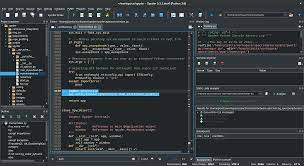
\includegraphics[width=4in]{figures/python_editor.jpg}
	\caption{Python IDE  \label{fig:python_editor}}
\end{figure}


\begin{figure}[ht]
	\centering
	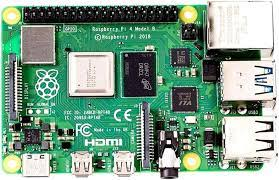
\includegraphics[width=4in]{figures/raspberi.jpg}
	\caption{Raspberry Pi.  \label{fig:raspberi}}
\end{figure}
   % include chapter 6 file

\chapter{Results \& Discussion}
The results (or findings) section is one of the most important parts of a research paper, in which an author reports the findings of their study in connection to their research question(s). The results section should not attempt to interpret or analyze the findings, only state the facts. In this handout, you will find a description of a results section, the differences between the results and discussion sections, differences between qualitative and quantitative data, sample results sections, and an activity to explore results in your field.  
\section{What is the Purpose of a Results Section?} 
The results section summarizes and presents the findings of the study to put them in context with your research question(s). The study’s data should be presented in a logical sequence without bias or interpretation. Findings may be reported in written text, tables, graphs, and other illustrations. It is important to include a contextual analysis of the data by tying it back to the research question(s). Only share relevant data and findings that connect with the goal of the study; too much data may overwhelm a reader. An effective results section will present the findings of a study without attempting to analyze or interpret them.
\section{How Does a Results Section Differ from a Discussion Section?}  

The results section of a research paper tells the reader what you found, while the discussion section tells the reader what your findings mean. The results section should present the facts in an academic and unbiased manner, avoiding any attempt at analyzing or interpreting the data. Think of the results section as setting the stage for the discussion section by making all the necessary information known to the reader. It is not uncommon for these sections to be combined, but researchers will often use sub-headings to distinguish between the two

\begin{figure}[ht]
	\centering
	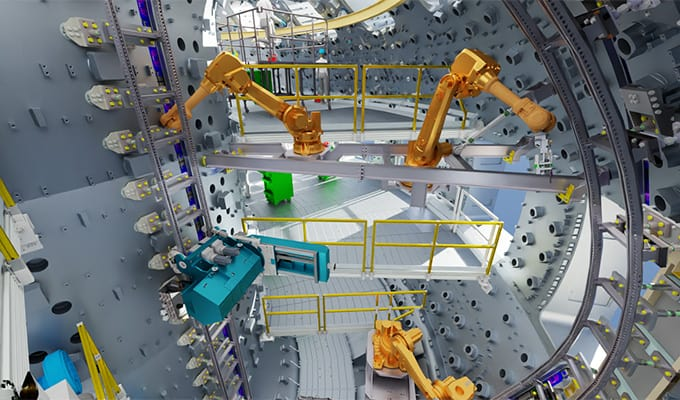
\includegraphics[width=4in]{figures/result_engg.jpg}
	\caption{Final Product\label{fig:over2}}
\end{figure}   % include chapter 7 file
\chapter{Conclusion}
%%
This chapter presents the results and conclusions of the project. It also contains a discussion on the cope of further research on the topic, on the social relevance of the project, and also the applicability of the findings of the project.
%%
\begin{table}[h]
	\centering
	\begin{tabular}{||c|c|c|c||}  \hline
		\hline
		Heading 1 & Heading 2 & Heading 3 & Heading 4  \\
		\hline \hline
		$D_{2,1}^{\nu}$ & $D_{2,2}^{\nu}$ & $D_{2,3}^{\nu}$ & $D_{2,4}^{\nu}$  \\
		\hline
		$D_{2,1}^{\nu}$ & $D_{2,2}^{\nu}$ & $D_{2,3}^{\nu}$ & $D_{2,4}^{\nu}$  \\
		\hline
		$D_{3,1}^{\nu}$ & $D_{3,2}^{\nu}$ & $D_{3,3}^{\nu}$ & $D_{3,4}^{\nu}$  \\
		\hline
		& & & \\
		\vdots & \vdots & \vdots & \vdots \\
		& & & \\
		\hline
		$D_{56,1}^{\nu}$ & $D_{56,2}^{\nu}$ & $D_{56,3}^{\nu}$ & $D_{56,4}^{\nu}$  \\
		\hline
		\hline
	\end{tabular}
	\caption{The sample table.\label{tab:1}}
\end{table}





\section{Scope of further work}
%%
\subsection{What is future direction in a project?}
The third element of your conclusion is a call to action or a future direction for your research paper. This is where you tell your readers what they should do or think based on your findings, or what you plan to do or explore next as a researcher.


   % include chapter 8 file
%\chapter{Final One}

This i sthe final added one

\section{intro to this chapter}

asssjhjhkjjj
\subsection{subsection}   % include chapter 9
file



%%
%% **********************************************************
%%
%% There is a file named references.tex. The file contains 
%% some sample references. Edit that file to include 
%% the details of the actual references.
%%
%% Bibliography with sample entries
%%
\newpage
%%
\renewcommand{\bibname}{References}
\addcontentsline{toc}{chapter}{\MakeUppercase{References}}
%%
%%
%%
\begin{thebibliography}{99}
%%
%% (Journal paper)

%%
%% (Referenced book)



\bibitem{Young}
{\bfseries G. O. Young}, Synthetic structure of industrial plastics, in {\em Plastics}, 2nd Ed., Vol.3,
J.Peters, Ed. New York: McGraw Hill, 1964, 15-64
%%
%% (Periodicals)

\bibitem{Bradshaw}
{\bfseries Bradshaw, P.},  An Introduction to Turbulence and its Measurement, Pergamon Press,
1971.

\bibitem{Duncombe}
{\bfseries J. U. Duncombe}, Inrared navigation – Part I : An Assessment of feasibility, {\em IEEE
Trans. Electron Devices}, Vol. ED-11, No.1, 34-39, Jan 1959
%%
%% (Reports)

\bibitem{CJ}Oxygen absorption in the earths

\bibitem{xx}
{\bfseries Bradshaw, P.},  An Introduction to Turbulence and its Measurement, Pergamon Press,
1111.

\bibitem{Reber}
{\bfseries E. E. Reber, R. L. Michell and C. J. Carter}, Oxygen absorption in the earths
atmosphere, Aerspace Corp., Los Angeles, CA, Tech. Rep. TR-0200 (4230-46)-3, Nov
1988.

\bibitem{Andrews}
{\bfseries Andrews, G.E and D.Bradley} (1972) The Burning Velocity of Methane-Air Mixtures,
{\em Combustion \& Flame}, 19, 275-288.

%%
%% (Manuals/Handbooks)
\bibitem{Report1}
Transmission Systems for Communications, 3rd Ed., Western Electric Co., Winston –
Salem, NC, 1985, 44-60.
\bibitem{Report2}
Motorola Semiconductor Data Manual, Motorola Semiconductor Products Inc.,
Phoenix, AZ, 1989.
%%
%% (Papers published in conference or symposium proceedings)
\bibitem{Lefebvre}
{\bfseries Lefebvre, A. H.}, (1965) Progress and Problems in Gas Turbine Combustion, {\em 10th
Symposium (International) on Combustion}, The Combustion Institute, Pittsburg, 1129-
1137.
%%
%% (On-line books)
\bibitem{Jones}{\bfseries Jones} (1991, May 10), Networks, (2nd Ed.) [Online]. Available: {\tt http://www.atm.com} (online journals).
\bibitem{Vidmar}
{\bfseries R. J. Vidmar}, (1992, Aug.). On the use of atmospheric plasmas as electromagnetic
reflectors. IEEE Trans. Plasma Sci. (Online).21(3), 876-880. Available:
{\tt http://www.halcyon.com/pub/journals/21ps03-vidmar}
\end{thebibliography}
%%
%%
%\appendix
%\achapter{Appendix 1}
%%
%% There is a file named publications.tex. The file contains 
%% some sample publications. Edit that file to include 
%% the details of the actual publications.
%%
%% List of publications with sample entries
%%
\newpage
%%
\renewcommand{\bibname}{List of Publications}
\addcontentsline{toc}{chapter}{\MakeUppercase{List of Publications}}
%%
%%
%%
\begin{thebibliography}{99}
%%
%% (Journal paper)
\bibitem{Andrews}
{\bfseries Andrews, G.E and D.Bradley} (1972) The Burning Velocity of Methane-Air Mixtures,
{\em Combustion \& Flame}, 19, 275-288.
%%
%% (Periodicals)
\bibitem{Duncombe}
{\bfseries J. U. Duncombe}, Inrared navigation – Part I : An Assessment of feasibility, {\em IEEE
Trans. Electron Devices}, Vol. ED-11, No.1, 34-39, Jan 1959
%%
%% (Papers published in conference or symposium proceedings)
\bibitem{Lefebvre}
{\bfseries Lefebvre, A. H.}, (1965) Progress and Problems in Gas Turbine Combustion, {\em 10th
Symposium (International) on Combustion}, The Combustion Institute, Pittsburg, 1129-
1137.
\end{thebibliography}
%%

\end{document}